\Chapter{RÉSULTAT EXPÉRIMENTAUX}\label{sec:Theme2}

Nous présentons les résultats en commençant d’abord par décrire l’implémentation du modèle conceptuel du robot logiciel codeur présenté dans la sous-section~\ref{subsection_cadre_conceptuel}. Ensuite, nous présenterons successivement les résultats propres à chacun des sous-objectifs décrits dans le chapitre~\ref{chapitre_methode}.

\section{Implémentation: du modèle conceptuel au modèle opérationnel}

L’implémentation de la machine (conceptuelle) est passée par la programmation manuelle d’une première interface et d’un premier noyau, en mettant à jour une version préliminaire de générateur basé sur une GUI\cite{bluiksnot_repo} en lui intégrant la capacité de générer du code à partir d’un module externe via son «hook» au moment de l’installation. La version à ce jour, ainsi que ses guides d’utilisation et ses scripts associés, sont disponibles sur le site de ERPLibre\footnote{\url{https://erplibre.ca}}.

L’interface permet l’interactivité avec un utilisateur ou le système-cible. L’interface est découplée en deux ensembles de méta-données: µ$_C^A$ et µ$_C^B$. µ$_C^B$ est l’ensemble qui paramétrise le passage de méta-données au code pour un module spécifique. µ$_C^A$ est l’ensemble qui paramétrise le passage de code aux méta-données tout en préparant un µ$_C^B$ adapté à ce module spécifique. Ce découplage a permis l’adaptation de l’interface au contexte de l’installation de modules sur une instance Odoo via des «hooks». Par la suite, un ensemble supplémentaire de méta-données, noté µ$_C^0$, a été dégagé de la programmation manuelle de versions successives de µ$_C^A$. µ$_C^0$ sert à initialiser une version de départ de µ$_C^A$.

Le noyau prend les paramètres issus de l’interface pour créer des méta-données, générer l’ensemble des fichiers des modules désirés (mode direct) et faire de la rétro-ingénierie (mode indirect) sur des modules existants.

\subsection{Développement et amélioration continue}

Dans la Figure~\ref{fig:dia_sequence_gc}, µ$_C^0$, µ$_C^A$, µ$_C^B$, C et M sont tous des modules installables sur Odoo. $M^i$ et $M^d$ sont des sections de code dans le module M. µ$_C^0$, µ$_C^A$ et µ$_C^B$ dépendent de M. µ$_C^A$, c’est les macro-méta-données, que µ$_C^B$, c’est les micro-méta-données.

\begin{figure}[htb]
\centering
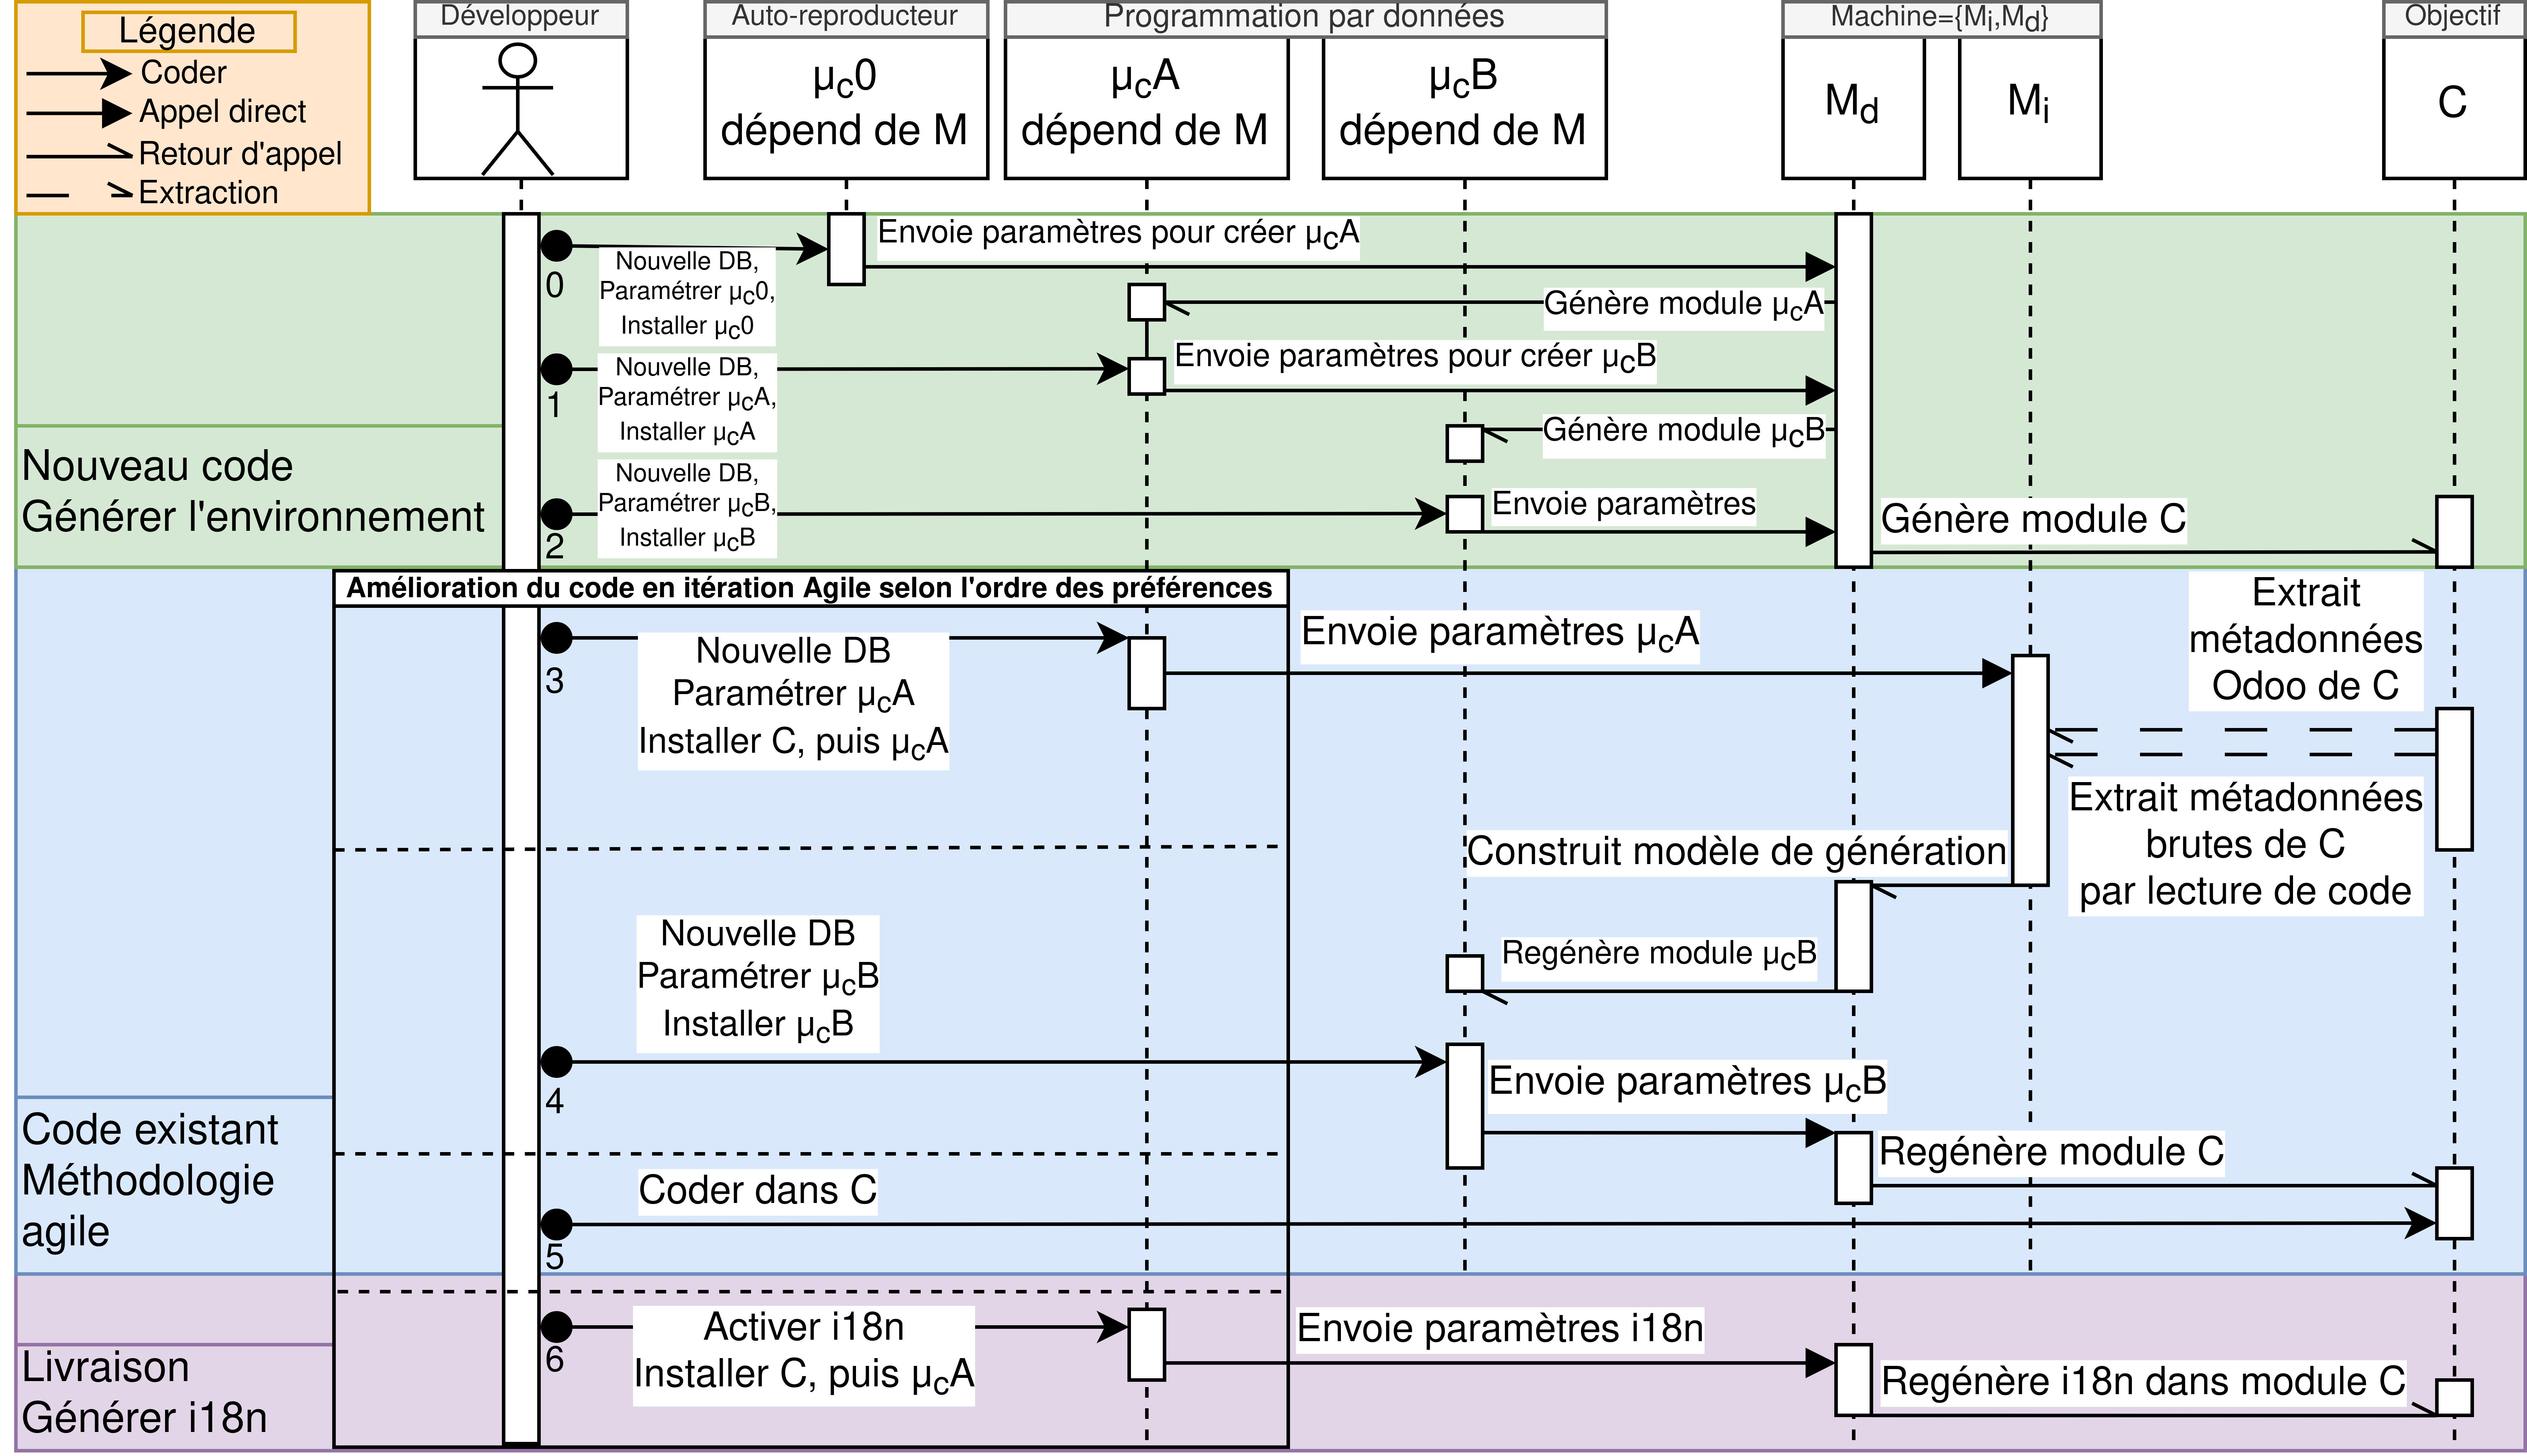
\includegraphics[width=6.535in]{images/code_generateur_erplibre_global_sequence.drawio.png}
\caption{Interaction du développeur avec le générateur de code}
\label{fig:dia_sequence_gc}
\end{figure}

Au départ d’un nouveau module code, µ$_C^0$ génère µ$_C^A$ qui génère µ$_C^B$ qui génère C. Il existe un script qui automatise un nouveau code, le développeur peut paramétrer le nom des modules et leurs emplacements. Ensuite, le développement commence en itération agile, les actions de 3 à 6 peuvent être exécutées dans l’ordre du choix du développeur.

% TODO expliquer raison/avantage de modifier soit µ$_C^A$, µ$_C^B$ ou le code directement.

Passer par l’étape 3 permet de mettre à jour l’étape 4 selon l’état du code via la rétro-ingénierie. Passer par l’étape 4 permet de mettre à jour le code selon le générateur. Il est possible de générer de nouvelles sections, comme la vue portail. Passer à l’étape 5 permet de personnaliser le code directement. Passer par l’étape 6 permet de mettre à jour le i18n de manière automatique.

La livraison sert à générer le i18n. C’est Odoo qui le génère, mais le générateur envoie les commandes, la liste des langues désirées à supporter et place les fichiers aux bons endroits dans le module. La raison pour laquelle c’est µ$_C^A$ qui doit le générer, c’est parce que le module doit être fini d’être généré et rechargé pour ensuite générer les langues, sinon ils sont corrompus par les traces de µ$_C^B$.

% TODO mettre dans discussion : Dans un contexte où l’ingénierie et la rétro-ingénierie serait parfaite, on n’aura pas besoin de mémoriser µ$_C^A$ et µ$_C^B$. Entre-temps, il y a une intervention humaine sur chacun de ces modules pour accélérer le développement. L’outil Git est utilisé pour faire des comparaisons entre les états d’itérations, seul ce qui est commité contient le bon contenu.

\subsection{Architecture}\label{architecture_result}

La Figure~\ref{fig:dia_architecture} démontre un développeur qui utilise l'interface de la machine qui opère dans le noyau de la machine.

\begin{figure}[htb]
\centering
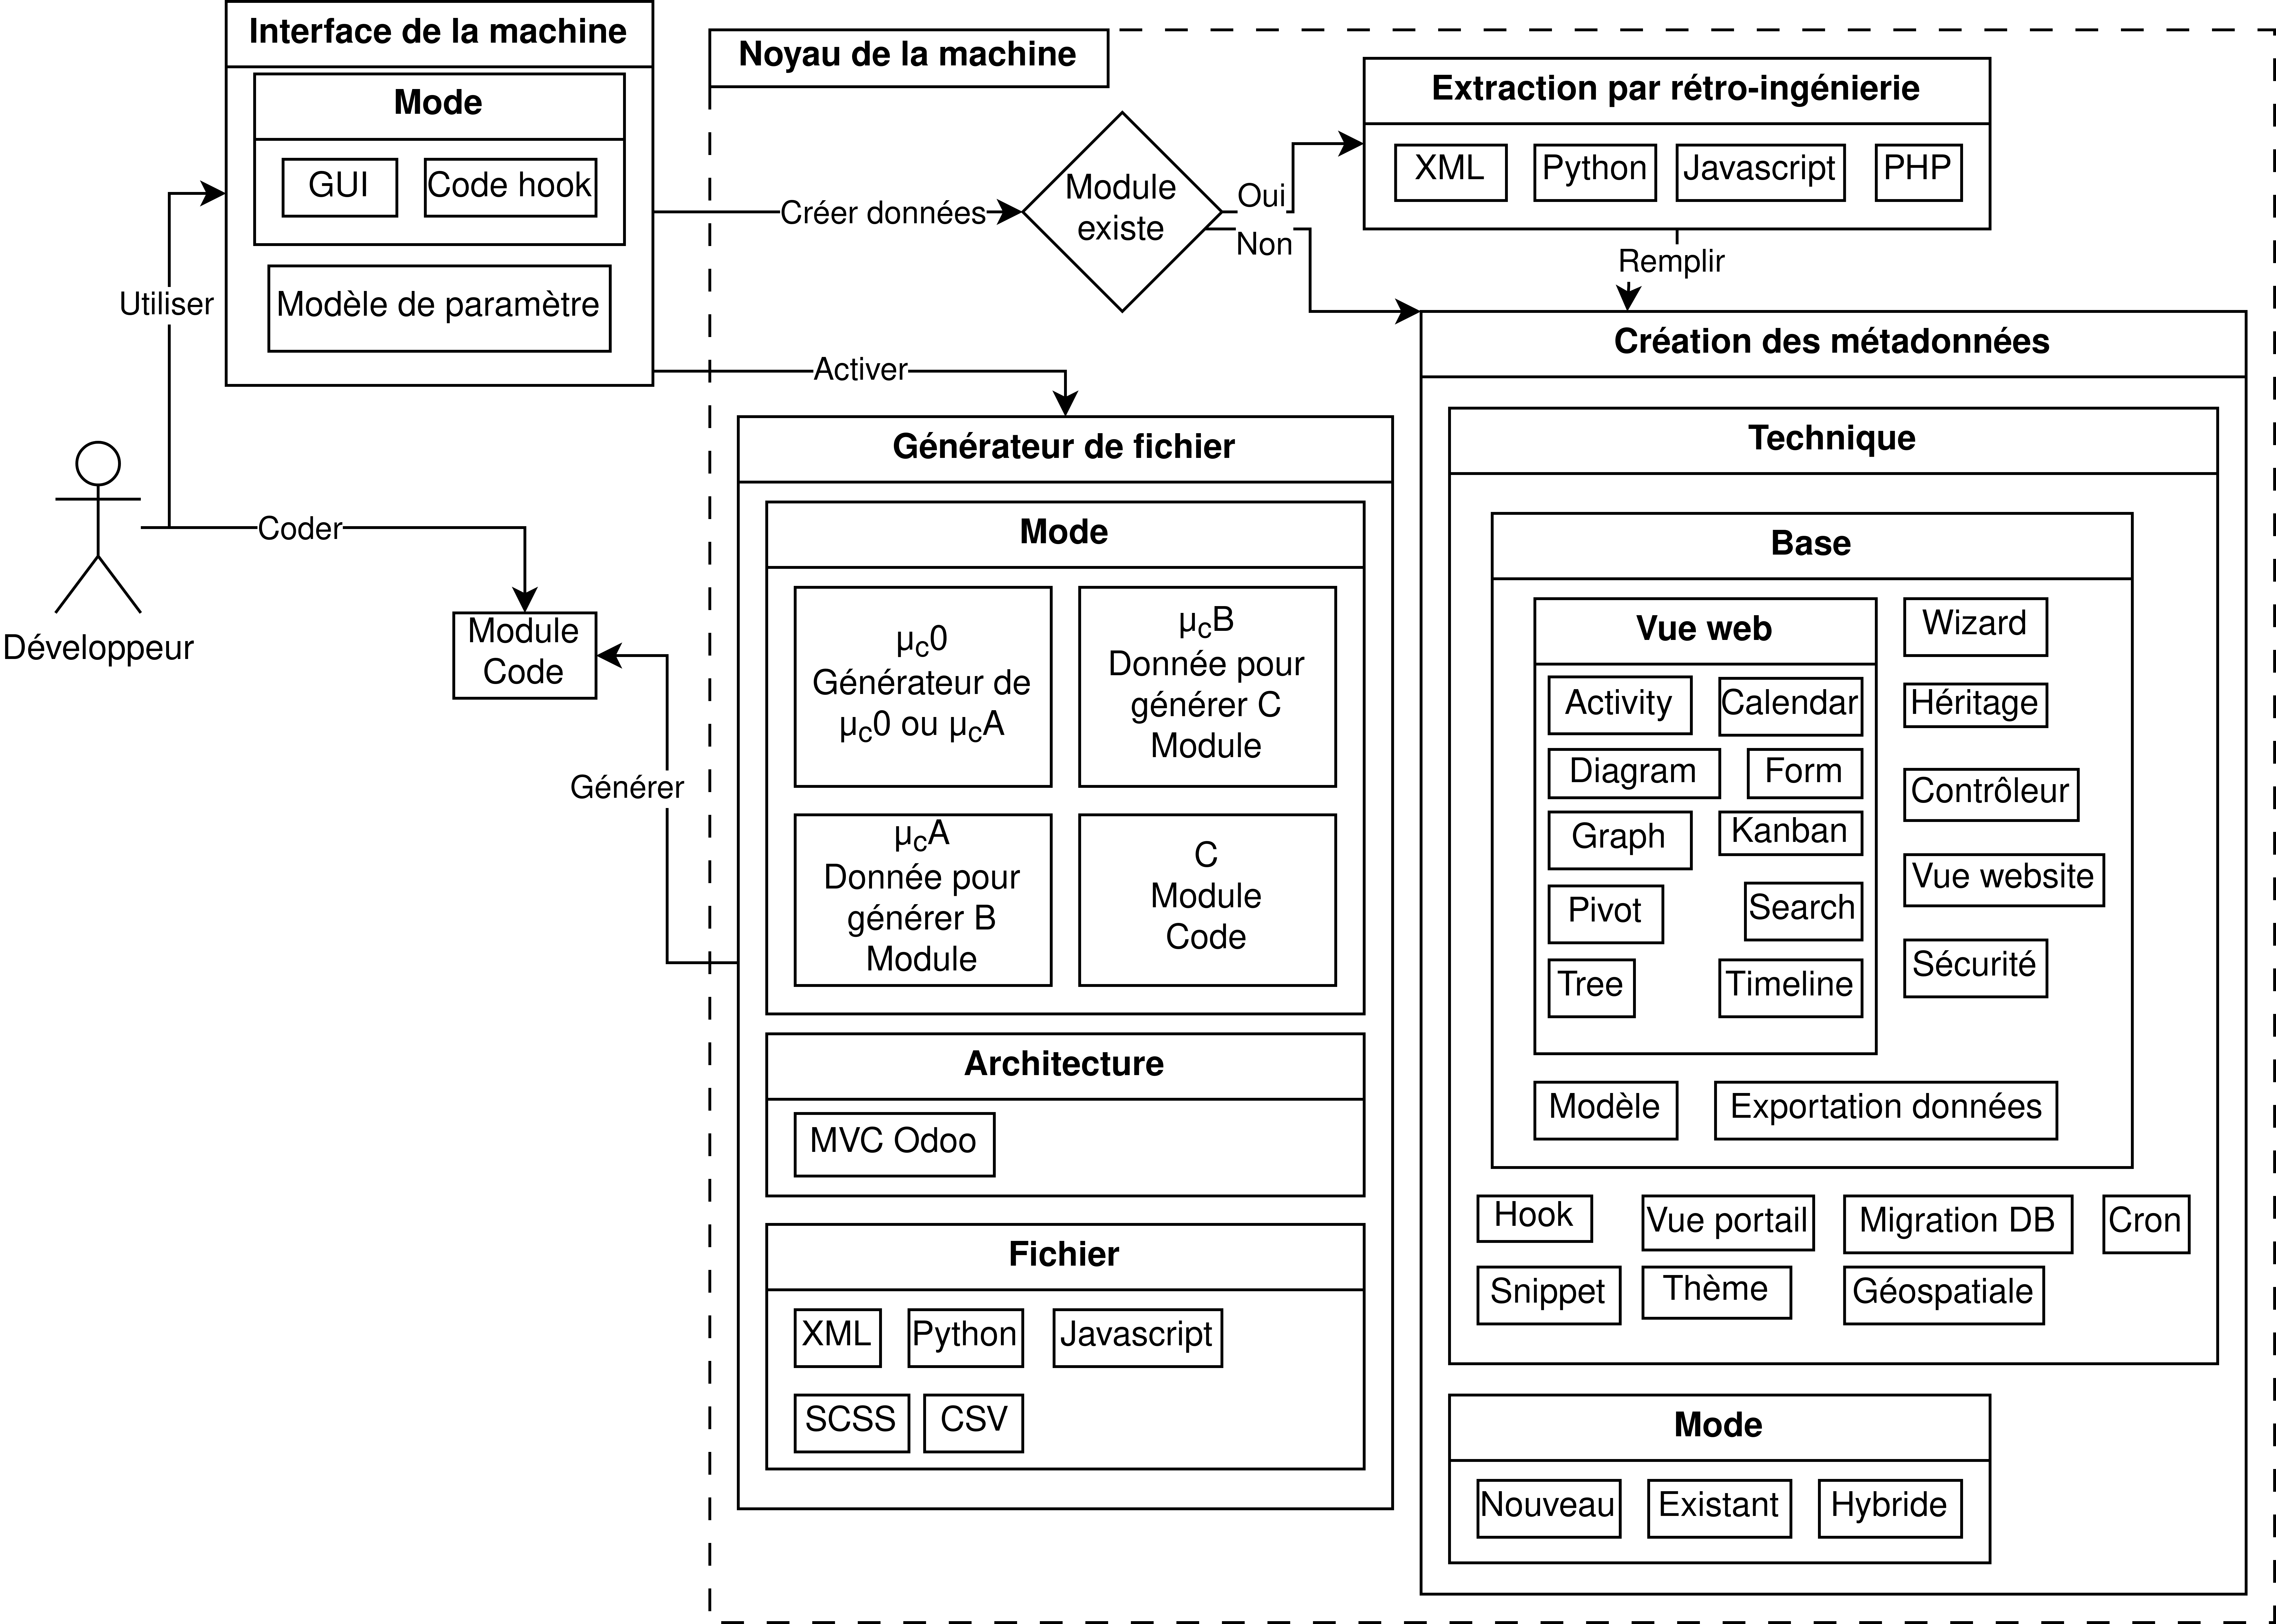
\includegraphics[width=6.535in]{images/architecture_machine.drawio.png}
\caption{Architecture du générateur de code dans son ensemble, nommé machine. Le développeur peut modifier le code source directement ou utiliser l'interface de la machine qui passe par un ensemble de composantes.}
\label{fig:dia_architecture}
\end{figure}

\begin{enumerate}
    \item L’interface machine permet à l’utilisateur de créer un modèle de données pour indiquer à la machine quelle opération effectuée avec leurs données associées. Plusieurs combinaisons, héritables, sont possibles selon les différentes techniques. De plus, c’est ici qu’on vient activer la génération de code.
    \item L’extraction par rétro-ingénierie permet de remplir le modèle de méta-données sans passer par la paramétrisation. Il extrait des informations qui ne sont pas accessibles dans le modèle de données d’Odoo sur le module.
    \item La création de méta-données se fait soit par l’utilisateur via la GUI ou le «Code Hook», il gère simultanément plusieurs techniques qui sont dans des modules. Le mode «nouveau» permet de créer de nouvelles données. Une fois qu’elles sont créées, c’est le mode «existant» qui est utilisé. Cependant le mode «hybride» permet d’écraser les données existantes en réactivant le mode «nouveau».
    \item Le générateur de fichier se fait activer par l’interface, mais il prend les méta-données pour faire sa génération selon le mode qu’il doit générer et l’architecture qu’il connaît. Il fait des liaisons entre les modèles et les vues en référence aux noms des champs de chaque modèle de données.
\end{enumerate}

Chacun de ces blocs de l’architecture est modulaire, chaque technique est héritable pour modifier le comportement et ajouter des liaisons pour permettre une génération de code au final.

La sécurité dépend du modèle. Le contrôleur dépend du modèle. La vue dépend du contrôleur et du modèle.

\subsection{Auto-générateur}

Représenté par µ$_C^0$, voir Annexe~\ref{annexe_cg_code_uc0}, c’est un auto-générateur! Au moment de son installation, il génère le même code que lui-même au même endroit dans le système de fichier. Une légère modification va créer une autre entité qui sera une déviation dans l’objectif de démarrer une chaîne.

C'est le module \texttt{M} qui contient les méta-données de µ$_C^0$. Ainsi, exécuter µ$_C^0$ devient un test de fonctionnalité et c'est un succès lorsqu'il n'y a pas de différence. Cependant sa programmation est actuellement spécifique à sa génération, aucun autre module n’a besoin de cette fonctionnalité unique.

% TODO TODO calcul code unique. HOW. Regarder le nombre de ligne exécuter avec ce module VS le nombre de ligne pour un autre module simple même type -> son µ$_C^A$ avec aucun modèle et un hook.
% TODO mettre référence vers le code

% Il pourrait être plus petit, faire appel à des méthodes extérieures. De plus, il pourrait y avoir moins de paramètre, on est pris entre la faciliter de paramétrer rapidement et la gestion de la lourdeur de beaucoup de paramètres. Présentement, la machine est limitée en fonctionnalité, mais plus que ça va avancer, plus il y aura de paramètres et il en aura trop pour tous les ajouter.

% TODO le terme chaine est nouveau, il faudrait le définir

L'auto-générateur est utilisé pour générer des µ$_C^A$ avec une légère modification dans les paramètres. Même s'il a la capacité de générer un µ$_C^B$, mieux vaut créer la chaîne proposée pour faire de l'amélioration continue.

\section{Résultats propres à SO-1}

\subsection{Génération par gabarit}

La génération par gabarit était déjà supportée dans la version initiale~\cite{bluiksnot_repo}, de plus, il y a eu des améliorations :
\begin{enumerate}
%TODO mettre en référence \footnote{\url{https://docs.python.org/3/whatsnew/3.6.html#pep-498-formatted-string-literals}}
    \item Utilisation des f-strings au lieu d'utiliser la fonction «format» de String.
    \item Utilisation de la bibliothèque Code-writer en Python\footnote{\url{https://pypi.org/project/code-writer/}}
    \item Utilisation de la bibliothèque lxml\footnote{\url{https://pypi.org/project/lxml/}}
\end{enumerate}

\subsection{MVC}

L’architecture MVC était déjà supportée dans la version initiale~\cite{bluiksnot_repo}, de plus, il y a eu des améliorations : 

\begin{enumerate}
% TODO define Wizard
 \item Ajout de bouton qui ouvre des «Wizard» pour générer les «Views», les «Models» et les «Controllers». Ainsi le développeur peut les configurer et demander de générer les méta-données associées.
    \begin{figure}[htb]
    \centering
    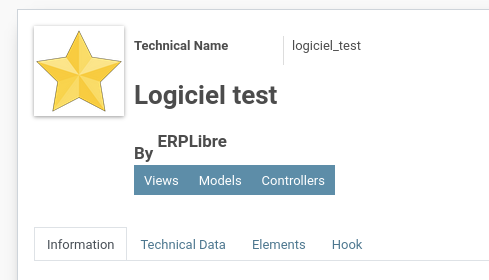
\includegraphics[width=3in]{images/GUI_MVC.png}
    \caption{Exemple support MVC dans GUI du générateur de code}
    \label{fig:dia_gui_mvc}
    \end{figure}
 \item Les règles de sécurité sont ajustées selon les configurations et personnalisables par la suite.
\end{enumerate}

\subsection{Générer un module à partir d’une base de données externes}

% Un module a été programmé pour suivre la technologie ETL
% TODO manque le load de https://fr.wikipedia.org/wiki/Extract-transform-load
% ça devient discussion

La migration de données à partir de SQL était déjà supporté dans la version initiale~\cite{bluiksnot_repo}, cependant il y a eu des améliorations : 

\begin{enumerate}
    \item Ajout de type de données, dont ceux utilisés par le projet Accorderie
    \item Ajout d'associations entre les types de données et les différentes personnalisations de l’architecture Odoo
    \item Interface représentant la base de données avec les contrôleurs permettant la configuration de la migration sur le modèle de données désirés
    \item Gestion des interdépendances (A de B et B de A)
\end{enumerate}

\subsection{Génération de code par des données}

La génération de code par des données a la capacité de prendre les données via les interfaces utilisateurs telles que la GUI et le «Code hook» Cela permet la personnalisation pour obtenir un logiciel adapté à ce que l’utilisateur est capable d’exprimer.

Le robot logiciel codeur est une machine qui grâce à son interface «code hook», se fait commander par deux couches de méta-données paramétrable par l’humain. Les deux couches s’interfèrent entre elles pour permettre l’évolution de la fonctionnalité désirée.

% TODO diagramme de couche entrée de l’utilisateur et sortie des fonctionnalités.

\subsection{Interprétation des résultats de SO-1}

\paragraph{SO-1 Accomplissements}
Simplification de l’écriture de technique dans le générateur de code avec l’utilisation de «f-string», de la bibliothèque «Code-writer» et de la bibliothèque «lxml».\\
Ajout de «Wizard» pour configurer le MVC selon des paramètres.\\
Amélioration de l’importation des bases de données externes.\\
Support de la génération de code par des données.\\
Augmentation de technique de génération de code, support des templates «Qweb», ajout du type de données géospatiale.

\paragraph{SO-1 Feuille de route}
Implémenter les fonctionnalités manquantes dans la GUI pour générer les MVC d’un module.\\
Augmenter le nombre de technologies à supporter l'importation des données.\\
Ajouter le support de génération sur différentes architectures.\\
Il manque des techniques de sécurité à personnaliser, comme l’anonymisation des données.\\
Générer automatiquement une documentation sur l’utilisation d’une technique. \\
Supporter la génération sur d’autres systèmes ERP libres tel que Tryton\footnote{\url{https://www.tryton.org}}.

\section{Résultats propres à SO-2}

\subsection {Extraction de code et reproduction}

De la macro et micro extraction ont été réalisés avec plusieurs techniques combinées.

Pour pouvoir faire de la reproduction, il a suffit de faire de la macro extraction, c'est-à -dire faire une recherche dans toutes les classes pour copier le contenu de chaque méthode pour le transformer en méta-données et pouvoir faire l’opération direct de générer le code qui a été copié. L’utilisation de l’AST a servi à déterminer quelle ligne de code était à découper pour les recopier.

Cependant, il était nécessaire dans certains contextes de faire de la micro extraction, comme : 
\begin{enumerate}
    \item L’extraction des noms des constantes, ils sont transformés en valeurs lors de l’exécution;
    \item L’extraction des commentaires, qui n’est pas supportée dans la bibliothèque AST de Python 3.7;
    \item L’extraction des décorateurs;
    \item L’extraction des paramètres et noms des méthodes/fonctions;
    \item Les méta-informations d’un modèle (description, nom, etc.)
\end{enumerate}

De plus, les vues ont été extraites dans le but d'obtenir des méta-données spécifiques qui caractérisent la reconstruction de la vue, ces données n’étaient pas accessibles dans les données d'Odoo.

Certaines informations ont été extraites dans le Javascript à l’aide de la bibliothèque «pyjsparser».

Pour l’extraction d'un projet externe d'une autre technologie, un extracteur de PHP a été développé via un «parser» de la communauté\footnote{\url{https://github.com/JameelNabbo/PHP-Parsers}}.

% TODO manque info sur le générateur de générateur de code
C'est en développant les techniques de génération de code qu'on réalise la reproduction. Un script a été développé pour accélérer l’écriture du générateur de code, ainsi qu'un générateur de générateur de code. Ensuite, le développeur peut le transformer légèrement pour prendre les paramètres des méta-données.

\subsection {Amélioration continue sur la génération}

Grâce à l’extraction des méta-données, dès que la technique de génération est bien développée avec les méta-données, le code est automatiquement généré avec de bonnes pratiques logicielles corrigeant automatiquement les problèmes.

L’intérêt de passer par Odoo pour lire le module valide déjà certains fonctionnements (par exemple : pas d’erreur de syntaxe dans le Python ou les XML étaient bien construits).

Ainsi, pour un module désiré, nous utilisons les outils pour générer µ$_C^A$ et µ$_C^B$, puis en avançant dans le développement, nous bouclons entre le 3 et 4 sur Figure~\ref{fig:dia_sequence_gc}.

\subsection {Test de validation de génération de codes}\label{test_validation_generation_code_resultat}

Pour tester ce générateur de code, la technique du test de comparaisons des sorties de la génération a été utilisé. Pour procéder, un développeur valide via l'outil Git ce qui est commité\footnote{Un terme dans l'outil Git pour valider le code en créant un état dans l'historique.}. Ainsi, un script a été développé pour lancer en parallèle les tests et valider les différences de génération avec ce qui a été commité précédemment. Aucune différence est un succès.

Il y a plusieurs types de test : 
\begin{enumerate}
    \item Valider l’installation du module généré;
    \item Valider que µ$_C^B$ génère bien le module cible sans différence dans le code;
    \item Valider que µ$_C^A$ génère bien µ$_C^B$ sans différence dans le code;
    \item L’extraction des paramètres et noms des méthodes/fonctions;
    \item Valider que la migration d’une base de données SQL se fait sans différence dans le code.
\end{enumerate}

En exécutant tous les tests, voir annexe~\ref{annexe_test_generateur_code}, une couverture de 84\% est obtenu, tous les tests présents sont un succès, sauf ceux sur l’auto-générateur.

\subsection {Règles de codage standardisées}

Au moment de générer les fichiers, toutes les sorties textes sont traitées par des outils de mise en forme en suivant des règles de codage standardisées.

Pour le Python, l’outil «black» est utilisé pour la mise en forme en suivant le standard PEP8 avec «isort» pour réordonner les importations. «black» donne une mise en forme non naturel comparé à l’écriture de code pour un humain, cependant, son résultat facilite la lecture et le suivi des différences pour les futurs ajouts.

Le Javascript, le HTML et le XML sont mise en forme avec l’outil «prettier».

De plus, le générateur force le déplacement des classes dans leur propre fichier respectif pour faire une classe par fichier.

Les champs pour chaque modèle sont déplacés en ordre alphabétique, mais le premier est celui qui est utilisé pour représenter le modèle\footnote{Référence à l'attribut «\_rec\_name»}.

\subsection{Interprétation des résultats de SO-2}

\paragraph{SO-2 Accomplissements}
Extraction du code via l’utilisation d’un AST et extraction des méta-données dans les fichiers XML.\\
Amélioration continue sur la génération de code grâce à la reproduction à l’aide de l’extraction du code.\\
Un outil pour aider à la création de technique de génération à l’aide d’un générateur de générateur de code.\\
Le générateur de code est accompagné de tests de validation en reproduisant l’ensemble des techniques en démonstration.\\
La génération de code applique des règles de codage standardisées.

\paragraph{SO-2 Feuille de route}
Finaliser l’implémentation de l'auto génération sur le robot logiciel codeur.\\
Mise à jour des tests pour atteindre une couverture de code à 100\%.\\
Ajout de test sur les techniques d’extractions de code tel que le PHP.

\section{Résultats propres à SO-3}

\subsection{Classification des techniques développées}\label{result_technique_developpe}

En référence à la Figure~\ref{fig:dia_architecture}, les techniques «Modèle», «Form», «Tree», «Contrôleur» et «Migration DB» étaient déjà implémentés dans la version initiale~\cite{bluiksnot_repo}, mais ils ont reçu des améliorations pour s’agencer aux autres techniques.

% TODO faire un diagramme des dépendances
Les techniques :
\begin{enumerate}
    \item Contrôleur;
    \item Cron;
    \item Exportation des données;
    \item Géospatiale (dépend de Modèle);
    \item Héritage;
    \item Hook;
    \item Migration DB\footnote{importation des données par DB};
    \item Modèle;
    \item Portal;
    \item Sécurité;
    \item Snippet;
    \item Thème;
    \item Vue web;
    \begin{enumerate}
        \item Activity;
        \item Calendar;
        \item Diagram;
        \item Form;
        \item Graph;
        \item Kanban;
        \item Pivot;
        \item Search;
        \item Timeline;
        \item Tree;
    \end{enumerate}
    \item «website\_leaflet» (dépend de Snippet et Géospatiale);
    \item Wizard;
\end{enumerate}

\subsection{Interface du générateur de code}

\paragraph{L'interface graphique}

 existait déjà dans la version initiale~\cite{bluiksnot_repo}, elle a été améliorée pour afficher plus d'informations par rapport aux développements. Elle sert à faciliter la paramétrisation du générateur de code. Elle n’a pas été priorisée et elle manque de fonctionnalités si on le compare à ce qui peut être supporté via la technique «code hooks» avec µ$_C^A$ et µ$_C^B$.

Ce qui fonctionne : 
\begin{enumerate}
    \item Créer un module;
    \item Renommer un module;
    \item Ajouter des modèles, voir Annexe~\ref{annexe_cg_gui_model}, et des champs, voir Annexe~\ref{annexe_cg_gui_champs};
    \item Ajouter des menus;
    \item Ajouter la sécurité;
    \item Changer les icônes;
    \item Changer les informations sur les propriétés «manifest» du module;
    \item Ajouter du code, voir Annexe~\ref{annexe_cg_gui_code};
    \item Modification des «hooks», voir Annexe~\ref{annexe_cg_gui_hook};
    \item Etc.
\end{enumerate}

\paragraph{L'interface «code hook»}

% TODO on montre un exemple de code hook?

permettent d’accéder à la totalité des fonctionnalités du robot logiciel codeur via µ$_C^A$ et µ$_C^B$, elles ont été utilisés pour toutes les démonstrations qui servent de test, elles contiennent la paramétrisation pour des modules désirés.

\subsection{Interprétation des résultats de SO-3}

\paragraph{SO-3 Accomplissements}
Ajout de nouvelles techniques et une classification de ceux-ci.\\
Rendre accessible une interface graphique pour paramétrer la génération de code.\\
Rendre accessible une interface de programmation pour utiliser toutes les fonctionnalités du robot logiciel codeur.

\paragraph{SO-3 Feuille de route}
Ajout de paramètres pour faire plus de personnalisation sur les techniques et les séparer une par module.\\
Supporter les fonctionnalités manquantes sur toutes les techniques pour l’interface graphique.\\
Supporter l’accès à la création de méta-données par la rétro-ingénierie via l’interface graphique.

\section{Résultats propres à SO-4}

\subsection{Utilisation d’un conteneur Docker}

Puisque le robot logiciel codeur fait partie de ERPLibre, la version 1.5.0 contient les modules de génération de code. Le déploiement se fait rapidement en utilisant le logiciel Docker, le générateur de code permet l’utilisation de l’interface graphique pour générer des modules Odoo.

\subsection{Interprétation des résultats de SO-4}

\paragraph{SO-4 Accomplissements}
Intégration dans un système de distribution via un Docker.

\paragraph{SO-4 Feuille de route}
Développer une synchronisation entre les instances pour permettre de la redondance.\\
Développer une gestion de son infrastructure via le générateur de code.\\
Faire participer le robot logiciel codeur à la maintenance de l’infrastructure de déploiement.\\
Utiliser d’autres systèmes de conteneur en distribution qui sont libres comme «Pod»~\footnote{\url{https://podman.io/}}.\\
le robot logiciel codeur doit avoir la capacité de valider techniquement si le logiciel est AGPLv3 au moment de l’exécution

\section{Résultats propres à SO-5}

\subsection{Guide : créer une communauté autour d’une technologie pour un réseau d’entraide libre}

Un guide hybride a été produit pour comprendre les aspects cités du démarrage d’un projet, de gestion d’une communauté autour d’un projet libre et des règles d'hébergement libres.

\subsection{Démarrage d’un projet}

Le guide du tableau~\ref{tab:demarrer_projet_7_etape} permet de démarrer rapidement un projet et s'assurer que les membres impliqués du réseau d'entraide comprennent les mêmes enjeux et s'alignent dans la même direction.

% TODO adapté selon le libre?

\begin{table}[htb]
\caption{Les 7 étapes pour démarrer un projet dans un réseau d'entraide}
\centering
\begin{tabular}{|l|l|}

\hline
\cellcolor[HTML]{d9d9d9}{\textbf{Étape}} &\cellcolor[HTML]{d9d9d9}{Description}\\\hline

\shortstack[l]{Mission} & \shortstack[l]{Trouver votre mission, vos indicateurs
% \footnote{\url{https://www.tresor.gouv.qc.ca/fileadmin/PDF/cadre_gestion/guide_indicateur.pdf}} 
et les objectifs associés.}\\\hline

\shortstack[l]{Processus} & \shortstack[l]{Déterminer les étapes pour du développement informatique, de \\ l'assemblage des travaux, des méthodes pour faire des services et de \\ l'amélioration continue.
\\Avoir conscience des gaspillages
% \footnote{\url{https://fr.wikipedia.org/wiki/Lean_(production)}}
}\\\hline

\shortstack[l]{Connexion} & \shortstack[l]{Mécanisme d'animation du suivi des tâches, des services.}\\\hline

\shortstack[l]{Valeurs} & \shortstack[l]{Trouver les valeurs qui vont guider la façon de gérer l'équipe, la \\ communauté, sans être exclusifs ou figées dans le temps. Ils sont \\ un point de repère et aide pour prendre les grandes orientations.}\\\hline

\shortstack[l]{Vision} & \shortstack[l]{Détailler un plan stratégique pour la communauté. C'est une \\ projection dans le futur pour permettre de comprendre la direction \\ sur la longue durée.}\\\hline

\shortstack[l]{Prochaines \\ étapes} & \shortstack[l]{Passer à l'action en mode itératif avec des méthodologies agiles.}\\\hline

\end{tabular}
\label{tab:demarrer_projet_7_etape}
\end{table}

\subsection{Intégration d’un membre}

\begin{enumerate}
    \item Amener les utilisateurs à faire des contributions en participant à la maintenance et en facilitant chaque étape d'implication;
    \item Rendre disponible des tâches pour les nouveaux membres;
    \begin{enumerate}
        \item Permettre d'utiliser des étiquettes de classement adaptés sur des initiatives proposé par des nouveaux, tels que «suggestion», «problème» ou «question».
    \end{enumerate}
    \item Remercier la personne pour son intérêt qui veut participer au projet;
    \item Répondre en moins de 24 heures pour accueillir le membre;
    \item Définir les types de contributions nécessaires et la manière qu'on examine une contribution;
    \item Mettre en place un sentiment d'appartenance :
    \begin{enumerate}
        \item Lorsqu'un problème est reporté, demander gentiment s'il peut avoir une contribution;
        \item Mettre la liste des contributeurs dans un fichier du projet;
        \item Remercier les contributeurs dans une infolettre.
    \end{enumerate}
    \item Émettre des dates de rencontres officielles pour parler du projet par vidéo-conférence pour des communautés locales, qui ont la même langue.
\end{enumerate}

\subsection{Comportement en communauté}

\begin{enumerate}
    \item Proposer un guide sur les comportements désirés;
    \item Réagir publiquement pour chaque message sur la plateforme;
    \item Encourager de publier les notes de réunions et même le menus commandés des repas pour promouvoir la transparence;
    \item Développer une culture de développement ouvert.
\end{enumerate}

\subsection{Outils de développement public}

\begin{enumerate}
    \item Mettre en place un site web de développement en lien avec l'organisation créé;
    \item Documenter publiquement le processus de développement;
    \item Permettre de voir l'avancement des tâches en lien avec les processus;
    \begin{enumerate}
        \item Permettre de proposer des changements avec un système d'acceptation par les pairs.
    \end{enumerate}
    \item Montrer la feuille de route du projet, des livrables prévues;
    \item Encourager la publication du travail brouillon avec un état de travail en progression;
    \item Déployer un moyen de discussion public et éviter de répondre en privé.
\end{enumerate}

\subsection{Résolution de problème}

\begin{enumerate}
    \item Mise en place d'un arbre décisionnel avec description des décisions sur un type de problème;
    \item Documenter la résolution d'un problème de développement logiciel;
    \item Permettre aux développeurs de prendre des décisions sur des choix impopulaires basés sur leur ressentiment;
    \item Éviter les débats réguliers sur des aspects triviaux;
    \item Concentrer les discussions vers la résolution d'un problème qui mène vers une action.
    \begin{enumerate}
        \item Quel serait la prochaine étape à prendre?
        \item Suggérer des conditions pour de nouveaux progrès, offrir un itinéraire, un chemin à suivre pour obtenir les résultats désirés.
    \end{enumerate}
\end{enumerate}

\subsection{Documentation}

\begin{enumerate}
    \item Rendre accessible les documentations :
    \begin{enumerate}
        \item Fonctionnelles pour les utilisateurs;
        \item Technique pour le développement;
        \item Hébergement pour le déploiement;
        \item Fichier «README» pour l'utilisation rapide du logiciel;
        \item Fichier «CONTRIBUTE» pour comment faire de la contribution;
        \item Fichier «GOVERNANCE» pour le départage décisionnel.
    \end{enumerate}
\end{enumerate}

\subsection{Sécurité}

\begin{enumerate}
    \item Montrer le niveau de sécurité de l'application;
    \item Mettre en place un système de communication des mises à jours nécessaires;
    \item Informer comment sécuriser les clés d'authentification, les données et les configurations personnelles.
\end{enumerate}

\subsection{Développement libre}

\begin{enumerate}
    \item Suivre les règles d'hébergement de logiciel libre pour permettre l'inclusion;
    \item Expliquer l'importance du choix de la licence libre ainsi que les différences. Expliquer pourquoi d'autres choix ne sont pas proposés et restreindre l'utilisation de logiciel libre si la licence n'est pas acceptée;
    \item Rendre accessible la documentation sur le logiciel libre en lien avec la localité administrative de l'organisation\footnote{Exemple, un document du Québec : \url{https://www.tresor.gouv.qc.ca/fileadmin/PDF/ressources_informationnelles/logiciels_libres/ll.pdf}};
    \item Toujours proposer des licences libres avec un guide explicatif, ne pas permettre d'utiliser des licences non compatible au libre :
    \begin{enumerate}
        \item LGPL3 et + - elle est acceptable, mais non désiré;
        \item GPL3 et + - pour toutes machines sans communication;
        \item AGPL3 et +\footnote{\url{https://www.gnu.org/licenses/agpl-3.0.en.html}};
        \item CC0\footnote{\url{https://creativecommons.org/share-your-work/public-domain/cc0/}}, ne protège pas l'oeuvre;
        \item CC-BY\footnote{\url{https://creativecommons.org/licenses/by/4.0/}};
        \item CC-BY-SA\footnote{\url{https://creativecommons.org/licenses/by-sa/4.0/}}, protège l'oeuvre;
        \item LiLiQ-R+\footnote{Licence libre restrictive au Québec : \url{https://forge.gouv.qc.ca/licence/}};
    \end{enumerate}
\end{enumerate}

\subsection{Communication}

\begin{enumerate}
    \item Faire un suivi des émotions/sentiments des membres lors des réunions (hebdomadaires) par rapport au projet;
    \item Mettre en place des outils favorisant la communication non violente.
\end{enumerate}

\subsection{Interprétation des résultats de SO-5}

\paragraph{SO-5 Accomplissements}
Test de la génération sur un module existant de la communauté nommé «auto\_backup».\\
Des modules de gestion de projet ont été générés pour faire le suivi de la conception fonctionnelle et de l’amélioration continue.\\
Le projet Accorderie a bénéficié du générateur de code pour la migration de la base de données vers Odoo.\\
Le projet Portail CEPPP a bénéficié du générateur de code pour la migration du code PHP vers Odoo, ainsi que de l’aide au développement de la section Portail.

\paragraph{SO-5 Feuille de route}
le robot logiciel codeur doit supporter la demande de «Pull Request» sur les projets Git respectif lorsqu’il y a une amélioration. Il doit faire le suivi et s’assurer de suivre les règles de contributions de la communauté.\\
Développer d’autres modules de gestion de projet pour l’accompagnement dans le développement de projet client.\\
Développer des modules de gestion de communauté sur des projets logiciels libres.\\
Développer le suivi du développement des modules communautaires avec une traçabilité sur les résultats avec des métriques de génie logiciel.

\section{Projets diverses}

\subsection{Projet module «auto\_backup»}

Le module «auto\_backup» est le premier module de la communauté à avoir été testé dans ce projet, un µ$_C^A$ et µ$_C^B$ a été généré et de la qualité a été appliqué causant une différence avec la version communautaire dans l’organisation OCA et leur répertoire «server-tools».

Ainsi, la technique de gestion des «Cron», puisqu’il lance des sauvegardes par SSH ou en local à des moments spécifiques dans le temps.

\subsection{Projet module workflow design}

C’est un module de gestion de projet généré par le robot logiciel codeur qui permet de faire le suivi sur les opportunités, les menaces, les forces, les faiblesses et les objectifs. Il a été utilisé dans le projet Accorderie.

\subsection{Projet module STARS}

Le module STARS dépend de l’application Projet, il permet de configurer une procédure associable à un nouveau projet pour suivre les étapes de STARS, voir Figure~\ref{fig:workflow_stars}.

\begin{figure}
\centering
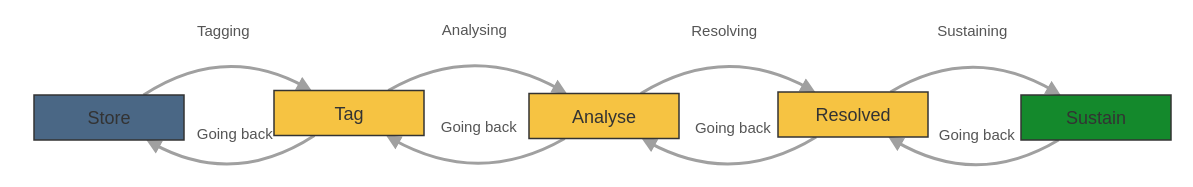
\includegraphics[width=6.535in]{workflow_stars.png}
\caption{Procédure STARS dans l'application Projet vue Diagramme}
\label{fig:workflow_stars}
\end{figure}

Ainsi, on peut créer un nouveau projet et suivre cette procédure en ajoutant des tâches d'amélioration continue de son organisation, voir Figure~\ref{fig:kanban_stars}.

\begin{figure}
\centering
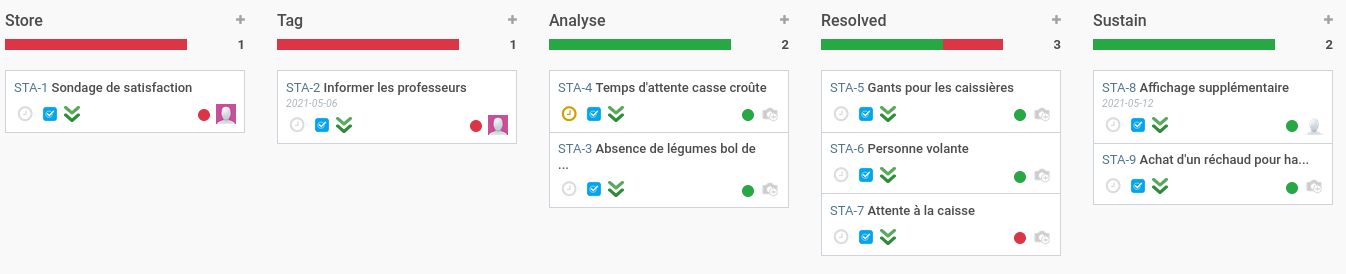
\includegraphics[width=6.535in]{kanban_stars.png}
\caption{Suivi des tâches de projet avec procédure STARS en vue Kanban}
\label{fig:kanban_stars}
\end{figure}

\subsection{Projet module SRS}

C’est un module de gestion de projet généré par le générateur de code qui permet de faire l’analyse des besoins pour ensuite passer à l’analyse fonctionnelle et finalement définir les requis fonctionnelles d’un projet. Il a été utilisé entre autre pour le projet Accorderie et le projet Portail CEPPP.

\section{Projet espace Accorderie}

Le projet a débuté par l'élaboration d'une analyse des besoins fonctionnels, puis un ensemble de requis logiciels ont été rédigés avec un membre du Réseau de l'Accorderie. % TODO faire annexe, voir annexe OIU.

Le générateur de code a permis de créer un module Odoo 12.0 avec leurs modèles de données basé sur leur base de données en SQL de MariadB, voir Annexe~\ref{annexe_db_accorderie_2019}.

Plusieurs corrections ont été effectuées avant la migration : correction des noms des champs pour les uniformiser; correction des types de champs (exemple le «True» était exprimé par la valeur «-1» dans un type «int», ainsi ce type a été transformé en booléen); enlever les doubles dépendances par changement de l’architecture; correction des données erronées (un champs est requis, mais il manque des données pour certaines entrées). De plus, le modèle de données n’a pas été conçue pour de l’automatisation, mais plutôt pour que les échanges de services soient validés par des membres de la communauté.

Dans l'Annexe~\ref{annexe_db_accorderie_2023}, on peut observer les adaptations des champs. Par exemple, avec la table «accorderie\_echange\_service», il y a l'ajout des champs : «nb\_heure\_estime» pour avoir une prévision des heures à effectuer, «nb\_heure\_dure\_trajet» pour reconnaître le temps de déplacement, «distance\_trajet» pour connaître la distance qui sera calculée avec le projet libre OSRM, etc...

La migration du modèle de données a été faite dans un module qui dépend de la technique «Migration DB» qui permet d'importer le modèle. Certaines données nécessitent la création d’un fichier de données XML. Pour les autres données, un autre module a été créé pour ajouter les données directement dans une base de données qui sera migré vers une mise en production.

Un portail a été généré, pour remplacer les formulaires utilisés par l'ancienne plateforme PHP pour visualiser les entrées. Cependant, cette fonctionnalité a été abandonnée puisque cette technologie ne plaisait pas.

Une maquette a été conçue pour un nouvel espace membre. Ainsi, nous avons utilisé la technique «website\_snippet» pour afficher des données sur le site web et créer des formulaires. Cette base a permis d’accélérer la création de code de communication entre le client et le serveur. À force de faire l’intégration et la personnalisation de cette maquette, il n’y a plus vraiment de code qui provient du générateur de code.

Le générateur de code a permis d’aider à créer un diagramme pour afficher le processus d’échange de temps, voir Annexe~\ref{annexe_processus_accorderie_2023}, puis une application en Javascript avec AngularJS a été développé pour afficher ce processus à l’utilisateur, une machine à état qui permet de revenir selon des paramètres à un état du processus.

Dû à des limitations humaines et de temps, tout le reste du projet a dû être fait manuellement puisqu’on a changé de technologie pour faciliter le développement de l’interface.

\section{Projet Portail CEPPP}

L'objectif est de faire une section portail pour les patients et une section administrative pour les recruteurs, les partenaires et les administrateurs de la plateforme, rendre accessible des formulaires et anonymiser les données. Le mandat était de migrer les fonctionnalités de la plateforme qui a été développée sur SuiteCRM en PHP.

Un module d'extraction de PHP a été développé, mais il n'est pas accessible dans les techniques du générateur de code. Le modèle de données était directement dans le code puisqu'il est dynamique, il n'est pas dans la base de données. La base de données n'a pas été extraite, les données ont été exportées en CSV et un module d'importation des données a été développé.

Extraction : 
\begin{enumerate}
    \item 23 fichiers analysés;
    \item 2851 données extraites;
    \item Capacité de faire la traduction anglais-français sur les données, mais cette fonctionnalité a été annulée puisque les données ont été modifiées dans la ré-ingénierie.
\end{enumerate}

Voici les statistiques~\ref{tab:stat_code_portail_ceppp} du code après ré-ingénierie et adaptation des fonctionnalités, livraison de la plateforme en début septembre 2023\footnote{\url{https://portailppp.ca}}.

\begin{table}[htb]
\caption{L'évolution entre la génération et la ré-ingénierie des statistiques sur les langages du portail CEPPP}
\centering
\begin{tabular}{|l|l|l|l|}

\hline
\cellcolor[HTML]{d9d9d9}{\textbf{Langage}} & \cellcolor[HTML]{d9d9d9}{\textbf{\# Ligne extrait}} & \cellcolor[HTML]{d9d9d9}{\textbf{\# Ligne personnalisé}} & \cellcolor[HTML]{d9d9d9}{\textbf{\# Diff}}\\\hline

XML & 6 861 & 3 856 & - 3 005\\\hline
Python & 567 & 1 564 & + 997\\\hline
Javascript & 0 & 68 & + 68\\\hline
CSV & 25 & 51 & + 26\\\hline

\end{tabular}
\label{tab:stat_code_portail_ceppp}
\end{table}

L'anonymisation n'est pas supportée par le générateur de code, puis la personnalisation enlève beaucoup de champs mis de manière générique dans les fichier XML. 

Le modèle de données du portail CEPPP dans Odoo 12 contient 24 modèles~\ref{annexe_db_ceppp_2022}. L'interface administrateur~\ref{annexe_form_ceppp_2022} contient la fiche du patient, que les partenaires ont accès seulement qu'à la partie anonymisée~\ref{annexe_form_anonyme_ceppp_2022}.

La signification que le nombre de lignes de XML aurait diminué, c’est que le générateur de code génère de base toutes les vues de tous les champs. Au moment de la ré-ingénierie, il y a eu beaucoup de nettoyage et de données XML effacées. Cependant, le développeur va mettre plus de code Python pour développer des logiques qui ne sont pas supportées par le robot codeur. Le Javascript ajouté sert à supporter les dates dans le portail. L’ajout de CSV sert pour l’ajout de permissions et rôles pour l’anonymisation.

\section{Comment les résultats obtenus soutiennent-ils le libre?}
Le réseau d’entraide a besoin d’un support technologie libre, puisque permettre aux participants de respecter leur 4 libertés vont permettre de pouvoir s’adapter à des situations d’urgence et apporter des solutions rapidement. Les 4 libertés sont :

\paragraph{Étudier}
La rétro-ingénierie a permis au le robot logiciel codeur de comprendre certaines fonctionnalités pour pouvoir recréer les méta-données adéquatement pour la reproduction.

\paragraph{Copier}
L’auto-générateur a été mis en place, il reste à auto-reproduire le robot logiciel codeur par son module principale de générateur de code.

\paragraph{Modifier}
Rend accessible la rétro-ingénierie tout en exécutant des mises en forme de code et de validation de la qualité logiciel.

\paragraph{Utiliser}
le robot logiciel codeur a la capacité d’utiliser ses fonctionnalités générées et d’exécuter des scripts d’automatisation à des périodes de temps adaptable.

\section{Avancement sur le réseau d'entraide}

\begin{figure}
\centering
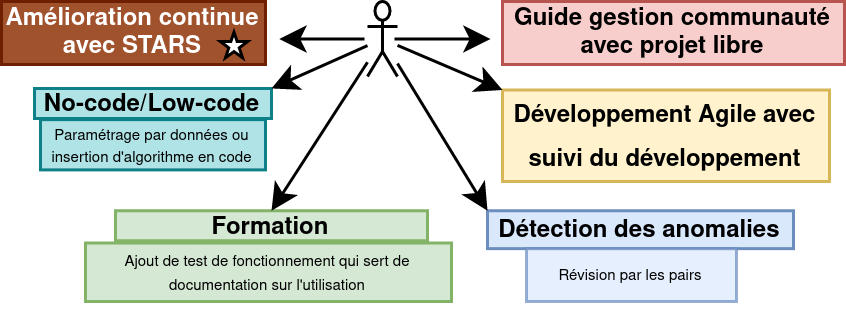
\includegraphics[width=6.535in]{images/developpeur_outil_developpement.drawio.png}
\caption{Intéraction entre le développeur et les outils de développement dans un réseau d'entraide}
\label{fig:dia_outil_dev_reseau_entraide}
\end{figure}

\section{Avancement de la technopoïèse}
% TODO résultat, séparer réseau d'entraide en développement
Avec la figure~\ref{fig:dia_auto_machine_discussion}, la ré-ingénierie manuelle est le processus habituel d'un développeur. Avec ce projet, nous avons une autopoïèse fonctionnelle semi-automatique, avec intervention humaine, puis une allopoïèse complète avec intervention humaine lorsque cette dernière est en dehors des techniques maîtrisées par le robot codeur. Le développement est au centre d'un réseau d'entraide avec des guides pour gérer son projet technologique.

\section{Réalisation du robot logiciel générateur de code}
% TODO résultat
Dans la revue littérature section~\ref{robot_logiciel_developpeur_revue}, nous avons déterminé 4 critères pour définir un robot codeur :
\paragraph{Autonomie}
Nous avons des résultats qui démontrent 100\% d'autonomie dans quelques contextes, voir les résultats sur les tests de validation section~\ref{test_validation_generation_code_resultat}. Cependant, le robot codeur n'est pas 100\% autonome pour tous les contextes, il a besoin d'intervention humaine pour des personnalisations ou des techniques non supportées.

% TODO une fois qu'on aura supporté plus de technique et l'autopoïèse entière, la prochaine étape serait de le faire fonctionner en continue. Bien qu'il soit capable via l'interface graphique, les efforts n'ont pas été effectué pour cette capacité.

\paragraph{Adaptable}
Le robot codeur est adaptable, il génère 6 composantes, voir résultat d'architecture section~\ref{architecture_result} : web, website, portail, snippet, migration de données entrants et migration de modèle de données entrantes. De plus, il est capable d'interagir avec des technologies en dehors d'Odoo telles que d'extraire du code externe en PHP du logiciel SuiteCRM et des bases de données externes (MySQL/SQL Server/PostgreSQL) pour importer des modèles de données et migrer des données.

% TODO il faudrait supporter la génération de technologies externes, nous travaillons présentement à générer des applications mobiles natives, ou même générer des modules sur d'autres plateforme ERP tel que Tryton ou NextERP.

\paragraph{Compétences techniques}
Le robot codeur contient plusieurs compétences techniques qui sont décrites dans les résultats section~\ref{result_technique_developpe}. De plus, il permet la personnalisation pour chacune des composantes du nombre de champs, des types de champs et du type d'affichage associé aux champs.

% TODO les techniques ont été développés comme preuve de concept, il manque de mâturité et de personnalisation. 

\paragraph{Compétences sociales}
Le robot codeur donne accès à des outils pour le développeur. Il y a une interface graphique LCNC qui permet la paramétrisation pour la génération de code. Il y a aussi une interface de code pour paramétrer le fonctionnement de la génération accompagnée de la rétro-ingénierie et il permet d'accompagner le développeur dans l'évolution de son module. Il contient aussi une fonctionnalité pour afficher les différences de code entre la version précédente et la version générée, il permet de créer des statistiques sur les lignes de codes, il permet de montrer la couverture de code, etc.

% TODO manque l'outil en temps réel, ce n'est pas supporté dans Odoo, il faut utiliser une application tierce tel que Etherpad et ajouter les méthodes de synchronisation des mises à jour sur les données. Il manque l'accès directe aux script à la racine du projet ERPLibre pour contrôler les outils de contrôle de la qualité. Collaboration, conscience professionnelle, résolutions de problèmes en équipe, communication efficace, adaptivité sur les livrables et exigences clientes

\begin{figure}
\centering
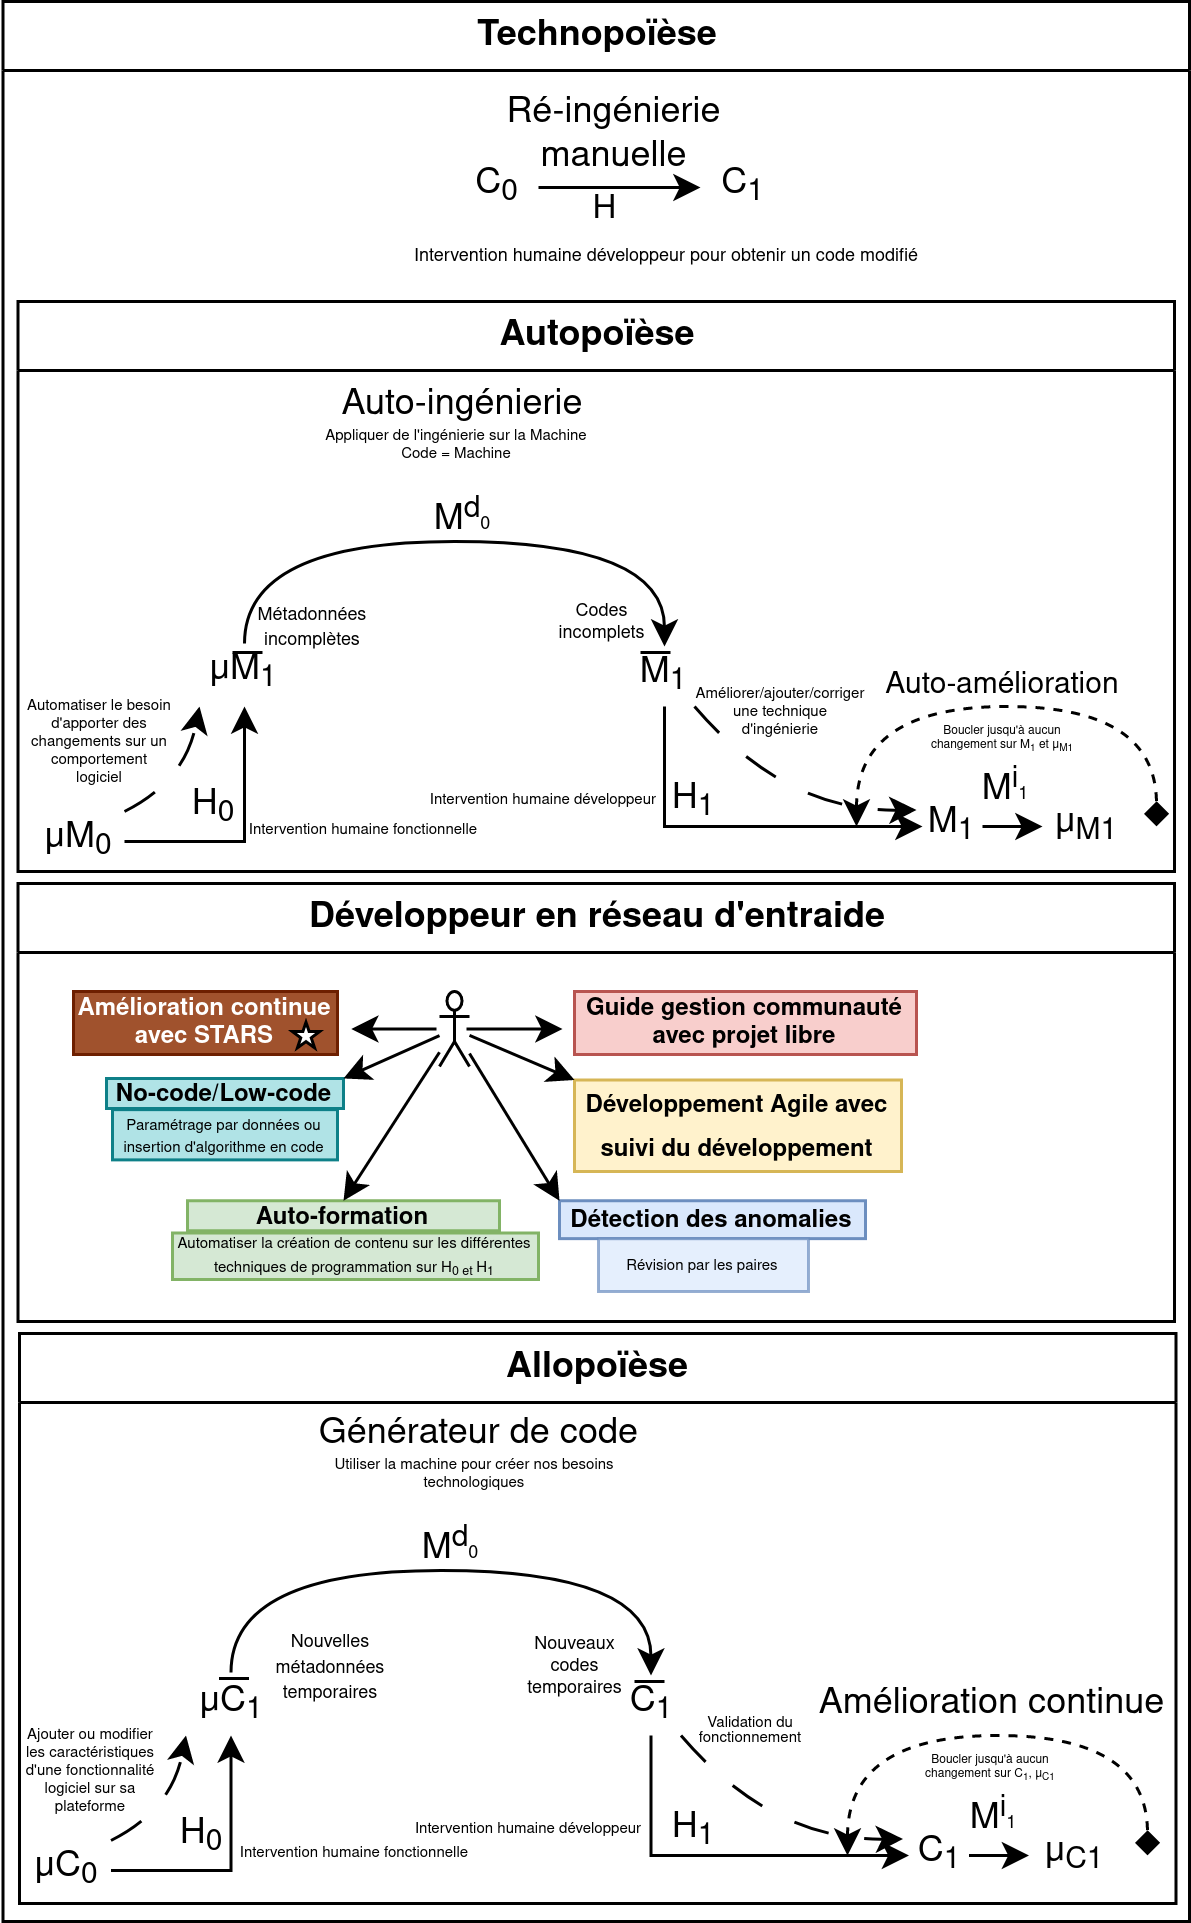
\includegraphics[height=8.5in]{images/auto_machine_discussion.drawio.png}
\caption{Architecture du générateur de code}
\label{fig:dia_auto_machine_discussion}
\end{figure}

% \subsection{DevOps}
% Il faudrait mettre en place les outils de dev ops.
% Mise à jour des bibliothèques (avoir une vue d’ensemble autre que Poetry)

% \subsection{Gestion de communauté}
% Un downtime de plus d’une journée cause drastiquement un abandon des participants à l’utilisation d’une technologie au sein d’une autre.

% \subsection{Réseau d’entraide}

% Il doit y avoir un responsable pour chaque localité accompagné du robot logiciel codeur pour répondre à ses besoins de numérisations via une souveraineté numérique. C’est le gestionnaire de communauté.

% Chaque projet d’urgence doit être capable d’avoir une équipe en charge pour accélérer la résolution de problèmes locaux.

% \subsection{Technopoïèse}
% À titre de discussion sur la signification de technopoïèse.

% Auto-répliqueur : une machine qui se copie lui même.
% Allopoïèse : une machine qui crée une autre machine avec des éléments extérieurs, l’inverse de l’autopoïèse.
% Autopoïèse : la propriété d’un système de se produire lui-même, en permanence et en intéraction avec son environnement, et ainsi de maintenir son organisation (structure) malgré son changement de composants (matériaux) et d’informations (données).
% REF https://fr.wikipedia.org/wiki/Autopo%C3%AF%C3%A8se
% Technopoïèse : une technologie qui a la propriété de se produire lui-même …
% «Une technologie pour étudier la vie humaine, des nouvelles sociétés et les accompagner dans leur développement d’autopoïèse. »
% La technopoïèse doit être développée dans un contexte de logiciel libre pour mettre au centre le réseau d’entraide et avoir le contrôle sur les dérives non éthiques.
% Outil passif utilisé par les humains pour jouer un rôle actif dans la création de la société et de la culture en façonnant leur environnement et leur mode de vie. Comprendre comment les technologies influencent la façon dont les individus interagissent et comment elles peuvent être utilisées pour améliorer la vie des gens, de manière responsable et éthique.

% \subsection{Robot codeur libre}

% Les robots codeurs peuvent être programmés pour effectuer différentes tâches, telles que la génération de code source, la correction de bugs, l'optimisation des performances, la maintenance des systèmes et la gestion de versions. Certains robots codeurs peuvent même apprendre à partir d'exemples de code existant et développer des algorithmes en se basant sur des données d'entrée.

% Les robots codeurs peuvent également améliorer la qualité du code en réduisant les erreurs humaines, en accélérant les tests et en appliquant des pratiques de codage cohérentes.»

% TODO projet d’impression 3D à distance, avec des propriétaires de machines qui les entretiennent.

% TODO connaissance de la physique et les appliquer, optimisation pour accompagner les communautés dans leur gestion d’urgence
% TODO doit reproduire les 4 libertés pour l’utilisation, l’accompagner dans son développement pour améliorer ses habitudes de vies par lui même sans dépendre d’autrui, restons en communauté locale pour réduire la consommation.
% TODO faciliter l’intégration de l’intération entre notre robot personnel et celui d’une technologie externe.

\subsection{Génération par gabarit}

L’utilisation de f-string et de la bibliothèque Code-writer permet de faciliter la lecture du développeur puisque le code du générateur se rapproche plus du résultat généré.

\subsection{Template de «A template-based code generator for web applications»}
Le code source de cette application «A template-based code generator for web applications» n’est pas accessible facilement au public, par conséquence, il sera difficile de comparer son efficacité du coté pratique. Mettons par exemple : elle ne dispose pas de ORM, elle ne fait pas de rétro-ingénierie, elle n'a pas été dédié pour une communauté.
